\documentclass{article}
\usepackage[T1]{fontenc}
\usepackage{lmodern}
\usepackage{graphicx}
\usepackage{amsmath,amssymb}
\usepackage[a4paper,margin=2cm]{geometry}
\usepackage[absolute,overlay]{textpos}
\setlength{\TPHorizModule}{1mm}
\setlength{\TPVertModule}{1mm}
\usepackage[indonesian]{babel}
\usepackage{hyperref}
\setlength{\emergencystretch}{2em}
% unit: Halaman 76

\begin{document}

% === Halaman 76 (llm) ===

% (tidak ada teks dari model)

% deskripsi: Screenshot kode program Python untuk fungsi EkstraksiPesan yang mengimplementasikan ekstraksi pesan menggunakan metode LSB (Least Significant Bit) dari sebuah citra stego.
% bbox normalisasi: [0.0580, 0.1050, 0.9410, 0.7960]
\begin{textblock*}{185.43mm}(12.18mm,31.18mm)
\noindent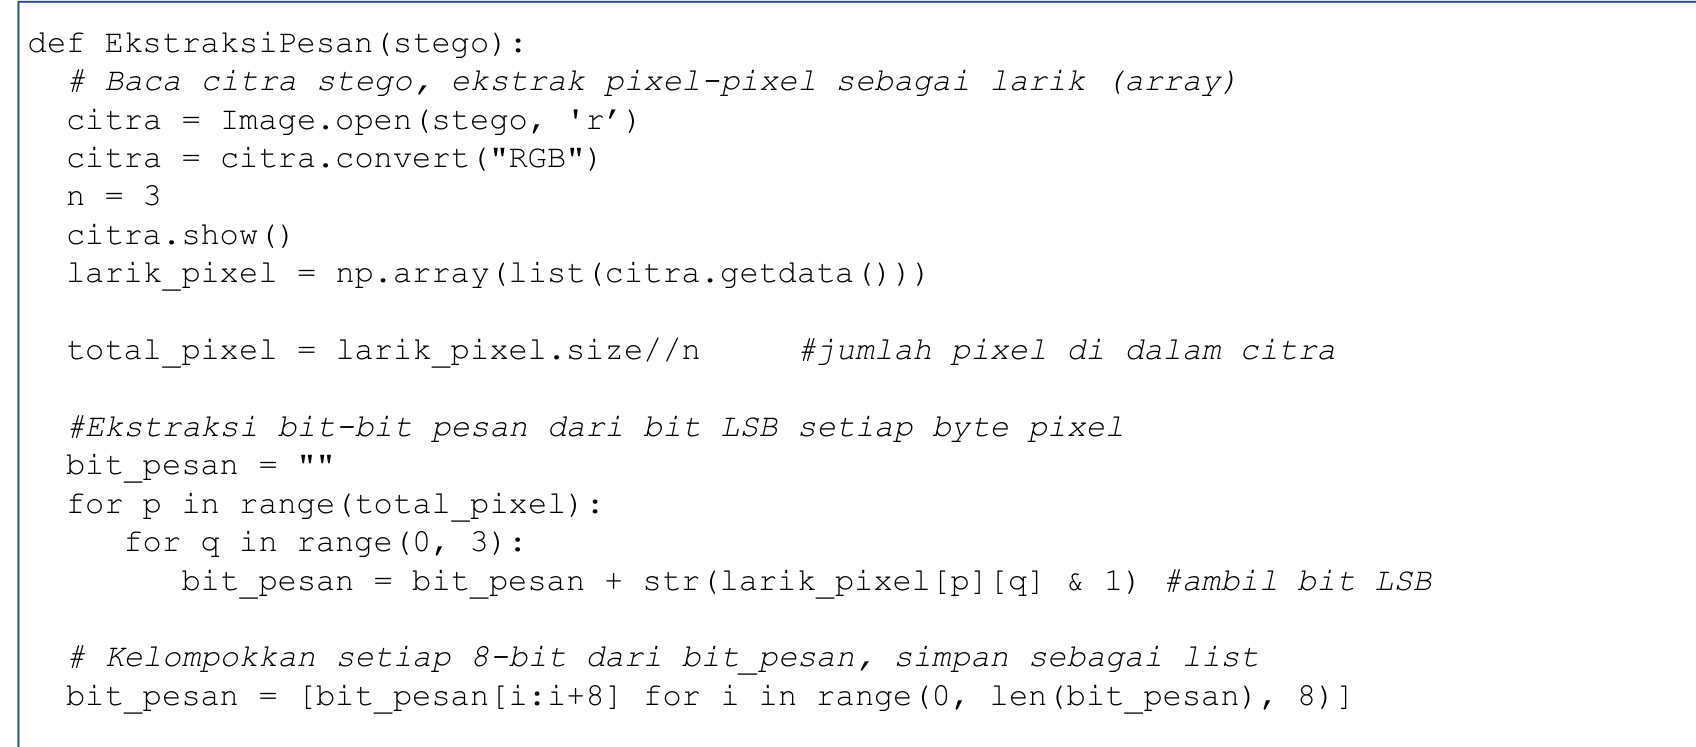
\includegraphics[width=185.43mm,height=205.23mm]{../../images/llm/page_076_img_01.png}%
\end{textblock*}

\end{document}
